\documentclass[10pt]{beamer} 
\usepackage{lmodern}
\setbeamertemplate{footline}[frame number]
\usepackage{graphicx}


%Information to be included in the title page:

\title{Domača Naloga 1}
\author{Enej Podlipnik, 23221334}
\institute{Fakulteta za strojništvo, Univerza v Ljubljani} 
\date{\today} 
\begin{document} 
\frame{\titlepage}

\begin{frame}
\frametitle{Kazalo}
 \tableofcontents[sectionstyle=show, subsectionstyle=show]
\end{frame}

\begin{frame} 
\section{Vsebina datoteke $naloga1\_1.txt$}
\frametitle{Vsebina datoteke $naloga1\_ 1.txt$}
\textbf{Podatki predstavljajo časovne korake v katerih smo merili moč P[W]}
\begin{itemize}
    \item Vsebina prve vrstice datoteke : Čas [s]
    \item Vsebina druge vrstice datoteke : Število vrstic in število podatkov v vrstici
\end{itemize}
\vspace{5pt}
\textbf{Za branje podatkov iz datoteke sem uporabil funkcijo $importdata$} :
\begin{itemize}
    \item Kot vhodne podatke funkcija vzame $datoteko$, $delimiterIn$ - pove kje v vrstici naj "razcepi" datoteko in pa $headlinesIn$ - pove, koliko vrstic naj funkcija preskoči na začetku, preden začne brati podatke.
    \item Kot izhod dobimo podatke, shranjene v vektor.
\end{itemize}
\end{frame}
\begin{frame} 


\section{Graf $P[t]$}
\frametitle{Graf $P[t]$}  
\vspace{10pt}
Graf P(t) izrisan iz podatkov dobljenih iz datotek $naloga1\_1.txt$ in $naloga1\_2.txt$.
\begin{figure}
    \centering
    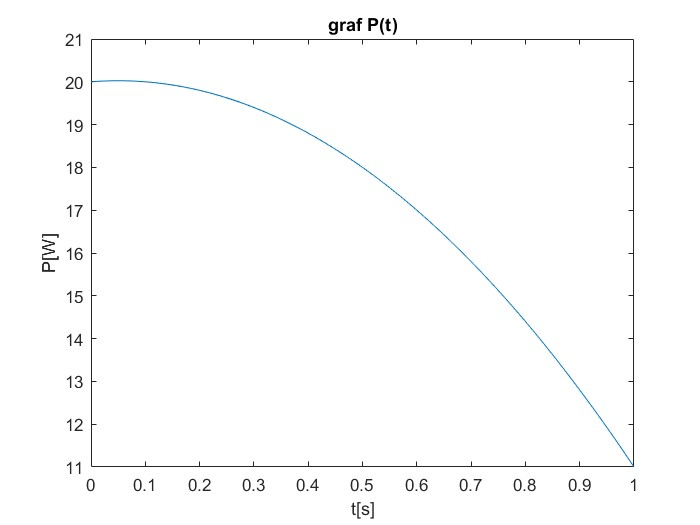
\includegraphics[width=0.9\linewidth]{grapP[t].jpg}
    \label{P(t)}
\end{figure}
\end{frame} 


\section{Trapezna metoda}
\begin{frame}[fragile]
\frametitle{Trapezna formula}
\begin{itemize}
   
\item Za izračun ploščine iz grafa [\ref{P(t)}], sem uporabil trapezno formulo:
$$\sum_{i=1}^{n-1} \frac{h_i}{2} (P_i + P_{i+1})\ ,$$

kjer $h_i$ predstavlja časovni korak : $h_i = t_{i+1} - t_i$. 

\item V Matlab-u sem formulo zapisal kot for loop:
\begin{verbatim}
result = 0;
for i = 1:1:(num-1)
    dt = t(i+1) - t(i); 
    s = dt/2 * (P(i) + P(i+1));
    result = result + s;
end
\end{verbatim}
\item \textbf{Rezultat izračuna je :} $17.1665\ J$
\end{itemize}
\end{frame}


\end{document}